\documentclass{beamer}
 
\usepackage[utf8]{inputenc}
\usepackage{svg}
\usepackage{tikz}
\usepackage{amsmath}
\usepackage[customcolors]{hf-tikz}
\usepackage[round]{natbib}

\usepackage{hyperref}
\usepackage{cleveref}
\usepackage{babel}
\usepackage{graphicx}



\definecolor{amber}{rgb}{1.0, 0.75, 0.0}
\definecolor{generator}{rgb}{0.67, 0.9, 0.93}
\definecolor{discriminator}{rgb}{0.89, 0.44, 0.48}
\definecolor{generated}{rgb}{0.82, 0.1, 0.26}
\definecolor{real}{rgb}{0.0, 0.5, 0.0}

\usetheme{metropolis}
 
 
\title[GAN]
{GAN - Theory and Applications}
  
\author
{Emanuele Ghelfi  \and \\ Paolo Galeone \and \\ Federico Di Mattia \and \\ Michele De Simoni}
 

 
\titlegraphic{
	 \begin{picture}(0,0)
	\put(100,15){\makebox(0,0)[rt]{
	
\includegraphics[height=1.2cm]{images/zuru-logo.png}}}
\end{picture}
}
 
 
 
\begin{document}
 
{
  \usebackgroundtemplate{
  	\tikz[overlay,remember picture] \node[opacity=0.2, at=(current page.center)] {
  		\includesvg[width=0.5\textwidth]{images/pycon_x_logo.svg}};}
  \begin{frame}
    \titlepage
  \end{frame}
}

 
\begin{frame}
	\frametitle{Generative Adversarial Networks}
	
	\setbeamercolor{block body}{bg=amber!20!white}
	\begin{block}{}
		{\large ``Adversarial Training (also called GAN for Generative Adversarial Networks) is the most interesting idea in the last 10 years of ML.''}
		\vskip5mm
		\hspace*\fill{\small--- Yann LeCun}
	\end{block}

\end{frame}

\begin{frame}
	\frametitle{Generative Adversarial Networks}
	
	Two components, the \textbf{generator} and the \textbf{discriminator}:
	\begin{itemize}
			\item The \textbf{generator} G, aim is to capture the data distribution.
			\item The \textbf{discriminator} D, estimates the probability that a sample came from the training data rather than from G.
	\end{itemize}
	
	\begin{figure}
		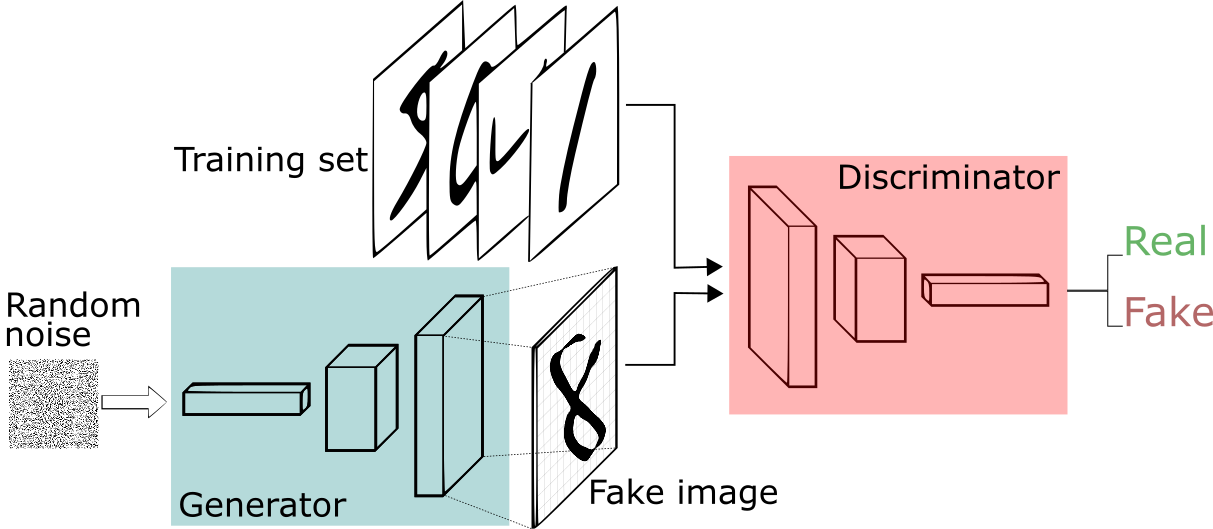
\includegraphics[width=0.9\textwidth]{images/GANs.png}
		\caption{Credits: \cite{silvaIntuitiveIntroductionGenerative2018} }
	\end{figure}

\end{frame}

\begin{frame}
	\frametitle{Generative Adversarial Networks}
	GANs game:
	\only<1>{
		\begin{equation}
		 \min_G \max_D V_{GAN}(D,G) = \underset{x \sim p_{data}(x)}{\mathbb{E}} [\log D(x)]  +\underset{z \sim p_z(z)}{\mathbb{E}}[\log(1 - D(G(z)))]
		\end{equation}
	}
	
	\only<2>{
			\begin{equation}
			\min_G \max_D V_{GAN}(D,G) =\color{real}\underbrace{ \color{black} \underset{x \sim p_{data}(x)}{\mathbb{E}} [\log D(x)]}_{\text{real samples}} \color{black}  +\underset{z \sim p_z(z)}{\mathbb{E}}[\log(1 - D(G(z)))]
			\end{equation}
	}
	
	\only<3>{
			\begin{equation}
			\min_G \max_D V_{GAN}(D,G) = \color{real} \underbrace{\color{black} \underset{x \sim p_{data}(x)}{\mathbb{E}} [\log D(x)]}_{\text{real samples}}  \color{black} + \color{generated} \underbrace{ \color{black} \underset{z \sim p_z(z)}{\mathbb{E}}[\log(1 - D(G(z)))]}_{\text{generated samples}} \color{black}
			\end{equation}
	}
\end{frame}

\begin{frame}
	\frametitle{GANs - Discriminator}
	Intuitive explanation:
	\begin{itemize}
			\item \textbf{Discriminator} needs to:
			\begin{itemize}
				\hfsetfillcolor{real!20}
				\hfsetbordercolor{real}
				\item Correctly classify \textcolor{real}{real} data: \\ 
					\begin{equation}
						\tikzmarkin{a}(0.2,-0.5)(-0.2,0.65)
							\max_D \underset{x \sim p_{data}(x)}{\mathbb{E}} [\log D(x)].
						\tikzmarkend{a}
					\end{equation}
				\item Correctly classify \textcolor{generated}{wrong} data: \\ 
					\hfsetfillcolor{generated!20}
					\hfsetbordercolor{generated}
					 \begin{equation}
						\hfsetbordercolor{discriminator} \tikzmarkin{b}(0.2,-0.5)(-0.2,0.65)
							\max_D  \underset{z \sim p_z(z)}{\mathbb{E}}[\log(1 - D(G(z)))].
						\tikzmarkend{b}
					 \end{equation}
		\end{itemize}
	\item The discriminator is an \textbf{adaptive loss function} that gets discarded once the generator has been trained.
	\end{itemize}
\end{frame}

\begin{frame}
	\frametitle{GANs - Generator}
	Intuitive explanation:
	\begin{itemize}
		\item \textbf{Generator} needs to \textbf{fool} the discriminator:
		\begin{itemize}
			\hfsetfillcolor{generated!20}
			\hfsetbordercolor{generated}
			\item Generate samples similar to the real one:
			\begin{equation}
				\tikzmarkin{c}(0.2,-0.5)(-0.2,0.65)
				\min_G  \underset{z \sim p_z(z)}{\mathbb{E}}[\log(1 - D(G(z)))].
				\tikzmarkend{c}
			\end{equation}
				\item Saturates easily \cite{goodfellowGenerativeAdversarialNetworks2014}.
				\item Change loss for generator:
					\begin{equation}
					\tikzmarkin{e}(0.2,-0.5)(-0.2,0.65)
					\max_G  \underset{z \sim p_z(z)}{\mathbb{E}}[\log( D(G(z)))].
					\tikzmarkend{e}
				\end{equation}
		\end{itemize}
	\end{itemize}
\end{frame}

\begin{frame}
	\frametitle{GANs - Models definition}
	\begin{itemize}
		\item Both D and G can be parametrized functions (Neural Networks).
		\item Different architectures for different data types.
		\begin{itemize}
			\only<1>{\item Tuple of numbers? \alert{Fully Connected Neural Networks}}
			\only<2>{\item Text or sequences?  \alert{Recurrent Neural Networks}}
			\only<3>{\item Images?  \alert{Convolutional Neural Networks}}
		\end{itemize}
	\end{itemize}

% figures
\only<1>{
		\begin{figure}
			\centering
			\includesvg[width=0.5\textwidth]{images/nn.svg}
		\end{figure}
}

\only<2>{
	\begin{figure}
		\centering
		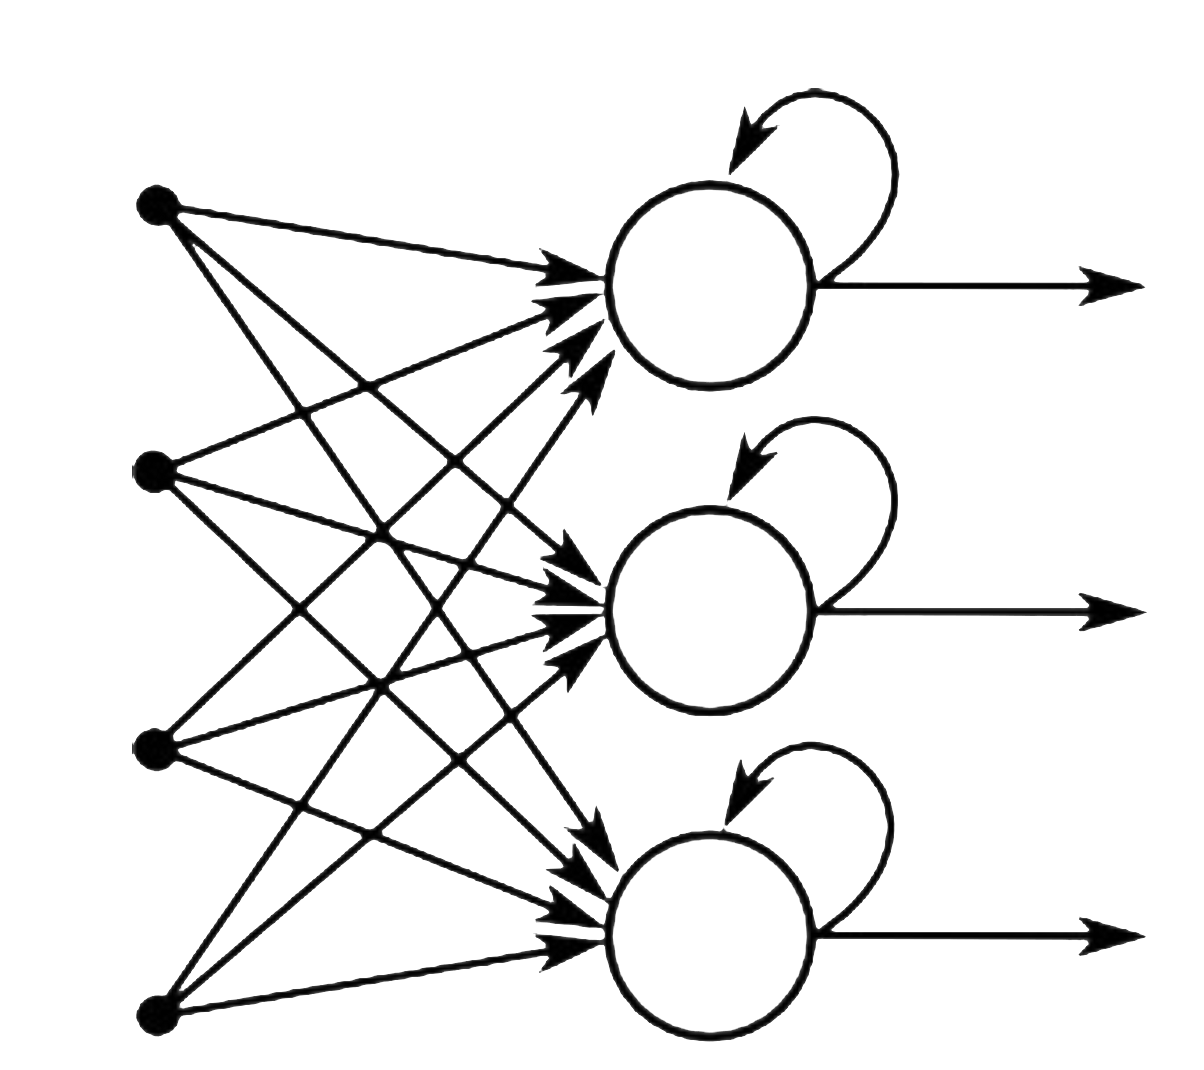
\includegraphics[width=0.5\textwidth]{images/recurrent.png}
	\end{figure}
}

\only<3>{
	\begin{figure}
		\centering
		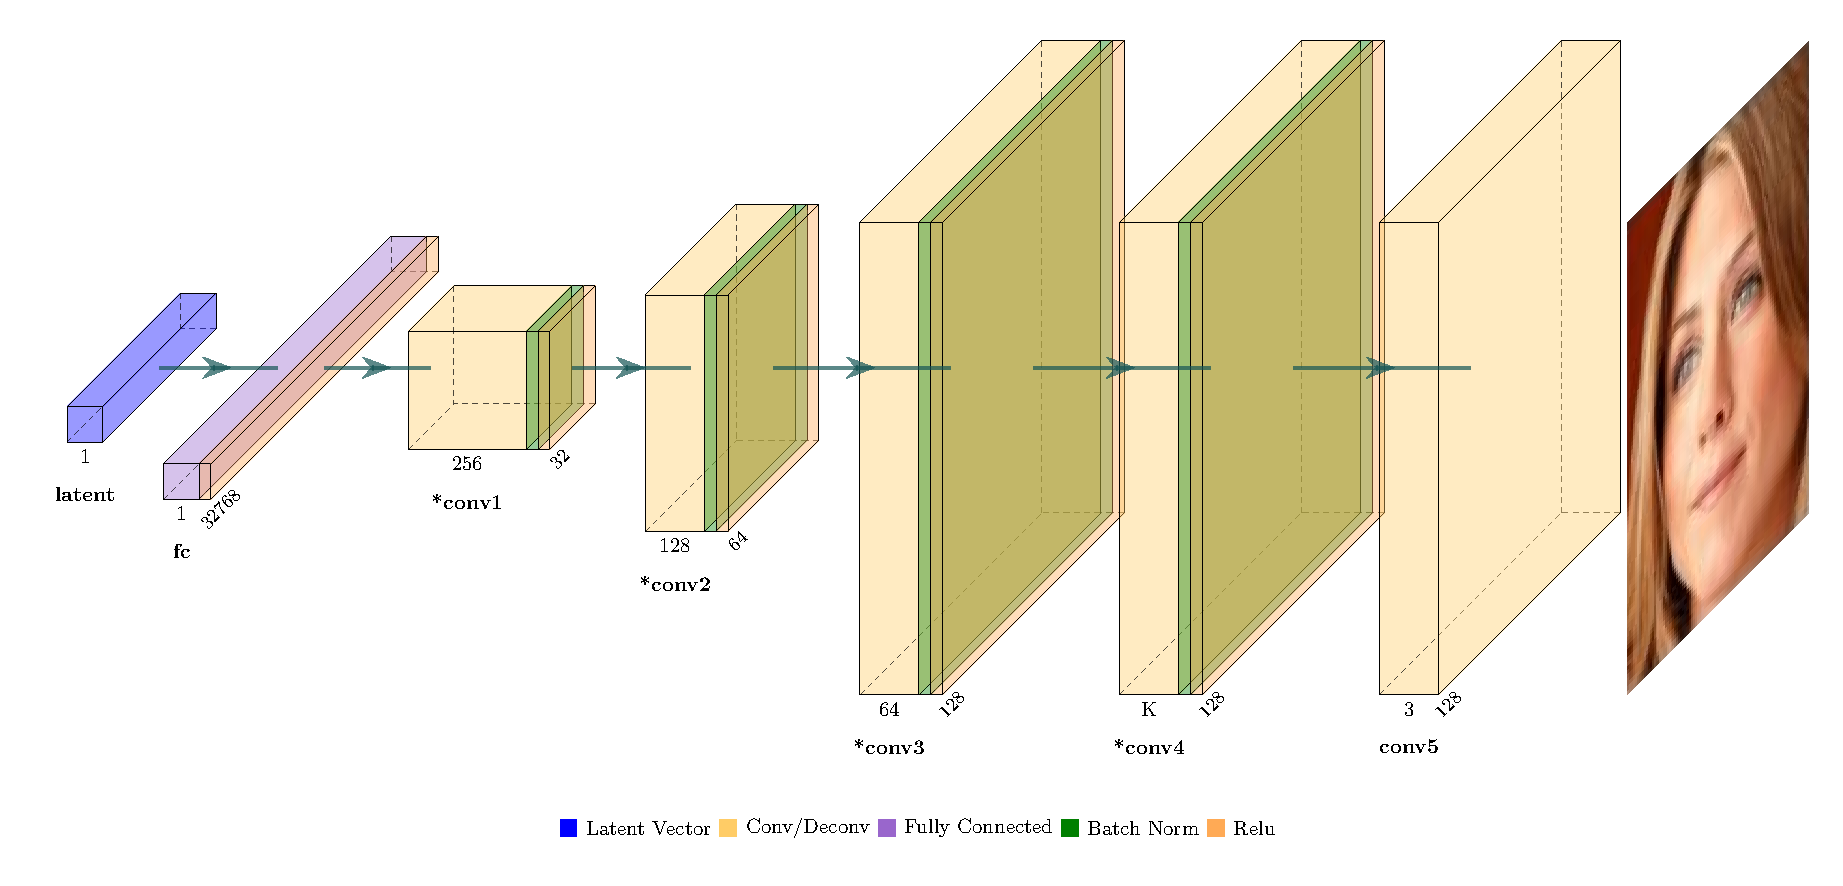
\includegraphics[width=0.9\textwidth]{images/cnn.pdf}
	\end{figure}
}
\end{frame}

\begin{frame}[standout]
	GANs Training
\end{frame}

\begin{frame}
	\frametitle{GANs - Training}
	\begin{itemize}
		\item Discriminator and generator are \textbf{competing} against each other.
		\item \textbf{Alternating} execution of training steps.
		\item Use \textbf{minibatch stochastic gradient descent/ascent}.
	\end{itemize}
	\begin{figure}
		\centering
		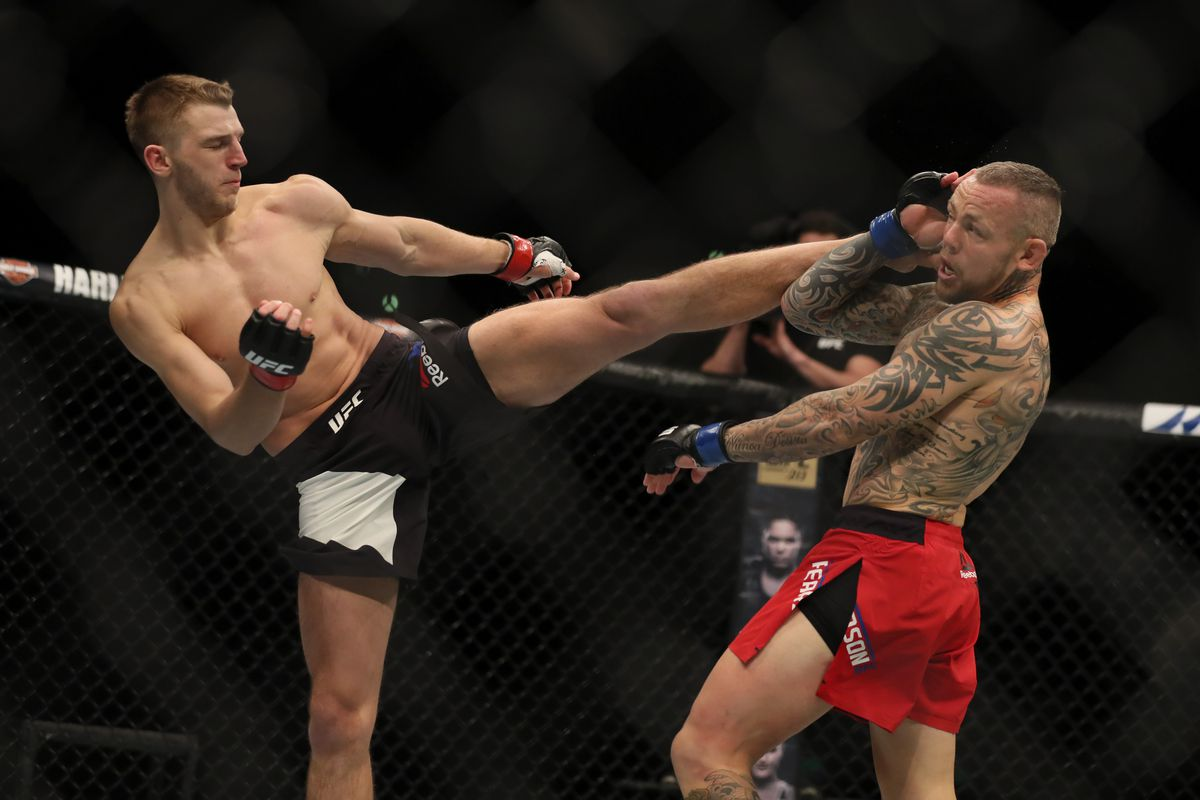
\includegraphics[width=0.7\textwidth]{images/fight.jpg}
	\end{figure}
\end{frame}

\begin{frame}
	\frametitle{GANs - Training - Discriminator}
	How to \textbf{train} the \textbf{discriminator}? \\
	Repeat from 1 to \textbf{k}:
		\begin{enumerate}
			\item Sample minibatch of $m$ noise samples ${z^{(1)},\dots,z^{(m)}}$ from $p_g(z)$
			\item Sample minibatch of $m$ examples ${x^{(1)},\dots,x^{(m)}}$ from $p_{data}(x)$
			\item Train the \textbf{discriminator} by stochastic gradient \textbf{ascent}:
	%		\only<1>{$$ \Delta_{\theta_d} \frac{1}{m} \sum_{i=1}^{m} \log D(x^{(i)}) + \log(1 - D(G(z^{(i)})))$$} 
	%		\only<2>{$$ \Delta_{\theta_d} \frac{1}{m} \sum_{i=1}^{m} \underbrace{\log D(x^{(i)}) + \log(1 - D(G(z^{(i)})))}_{\text{Discriminator loss}} $$
	%		}
		$$
			\nabla_{\theta_d} \underbrace{\frac{1}{m} \sum_{i=1}^{m} \underbrace{\log D(x^{(i)}) + \log(1 - D(G(z^{(i)})))}_{\text{Discriminator loss}}}_{\text{Loss estimation using m samples}}
		$$
		\end{enumerate}
\end{frame}

\begin{frame}
	\frametitle{GANs - Training - Generator}
	How to \textbf{train} the \textbf{generator}? \newline
	The update is executed \textbf{only once} and only after the turn of the discriminator is completed:
	\begin{enumerate}
		\item Sample minibatch of $m$ noise samples ${z^{(1)},\dots,z^{(m)}}$ from $p_g(z)$
		\item Train the \textbf{generator} by stochastic gradient \textbf{ascent}:
	%	\only<1>{$$ \Delta_{\theta_g} \frac{1}{m} \sum_{i=1}^{m} \log(D(G(z^{(i)})))$$}
	%	\only<2>{$$ \Delta_{\theta_g} \frac{1}{m} \sum_{i=1}^{m} % \underbrace{\log(D(G(z^{(i)})))}_{\text{Generator loss}} $$}
			$$
			\nabla_{\theta_g} \underbrace{\frac{1}{m} \sum_{i=1}^{m} \underbrace{\log(D(G(z^{(i)})))}_{\text{Generator loss}}}_{\text{Loss estimation using m samples}}
			$$
	\end{enumerate}
\end{frame} 

\begin{frame}
	\frametitle{GANs - Training - Considerations}
	\begin{itemize}
		\item Optimizers: Adam, Momentum, RMSProp.
		\item Training phase can last for an \textbf{arbitrary number} of steps or epochs.
		\item Training is completed when the discriminator is \textbf{completely fooled} by the generator.
		\item Goal: reach a \textbf{Nash Equilibrium} where the best D can do is random guessing.
	\end{itemize}
 \end{frame}

\begin{frame}[standout]
	Types of GANs
\end{frame}

\begin{frame}
	\frametitle{Types of GANs}
	Two big families:
	\begin{itemize}
		\item \textbf{Unconditional} GANs (just described).
		\item \textbf{Conditional} GANs \citep{mirzaConditionalGenerativeAdversarial2014}.
	\end{itemize}
\end{frame}

\begin{frame}
	\frametitle{Conditional GANs}
	\begin{itemize}
		\item \textbf{Both} $G$ and $D$ are \textbf{conditioned} on some extra information $ \color{red} y$.
		\item In \textbf{practice}:  perform conditioning by feeding $\color{red} y$ into the discriminator and generator.
	\end{itemize}
	\vspace{-1cm}
	\begin{figure}
		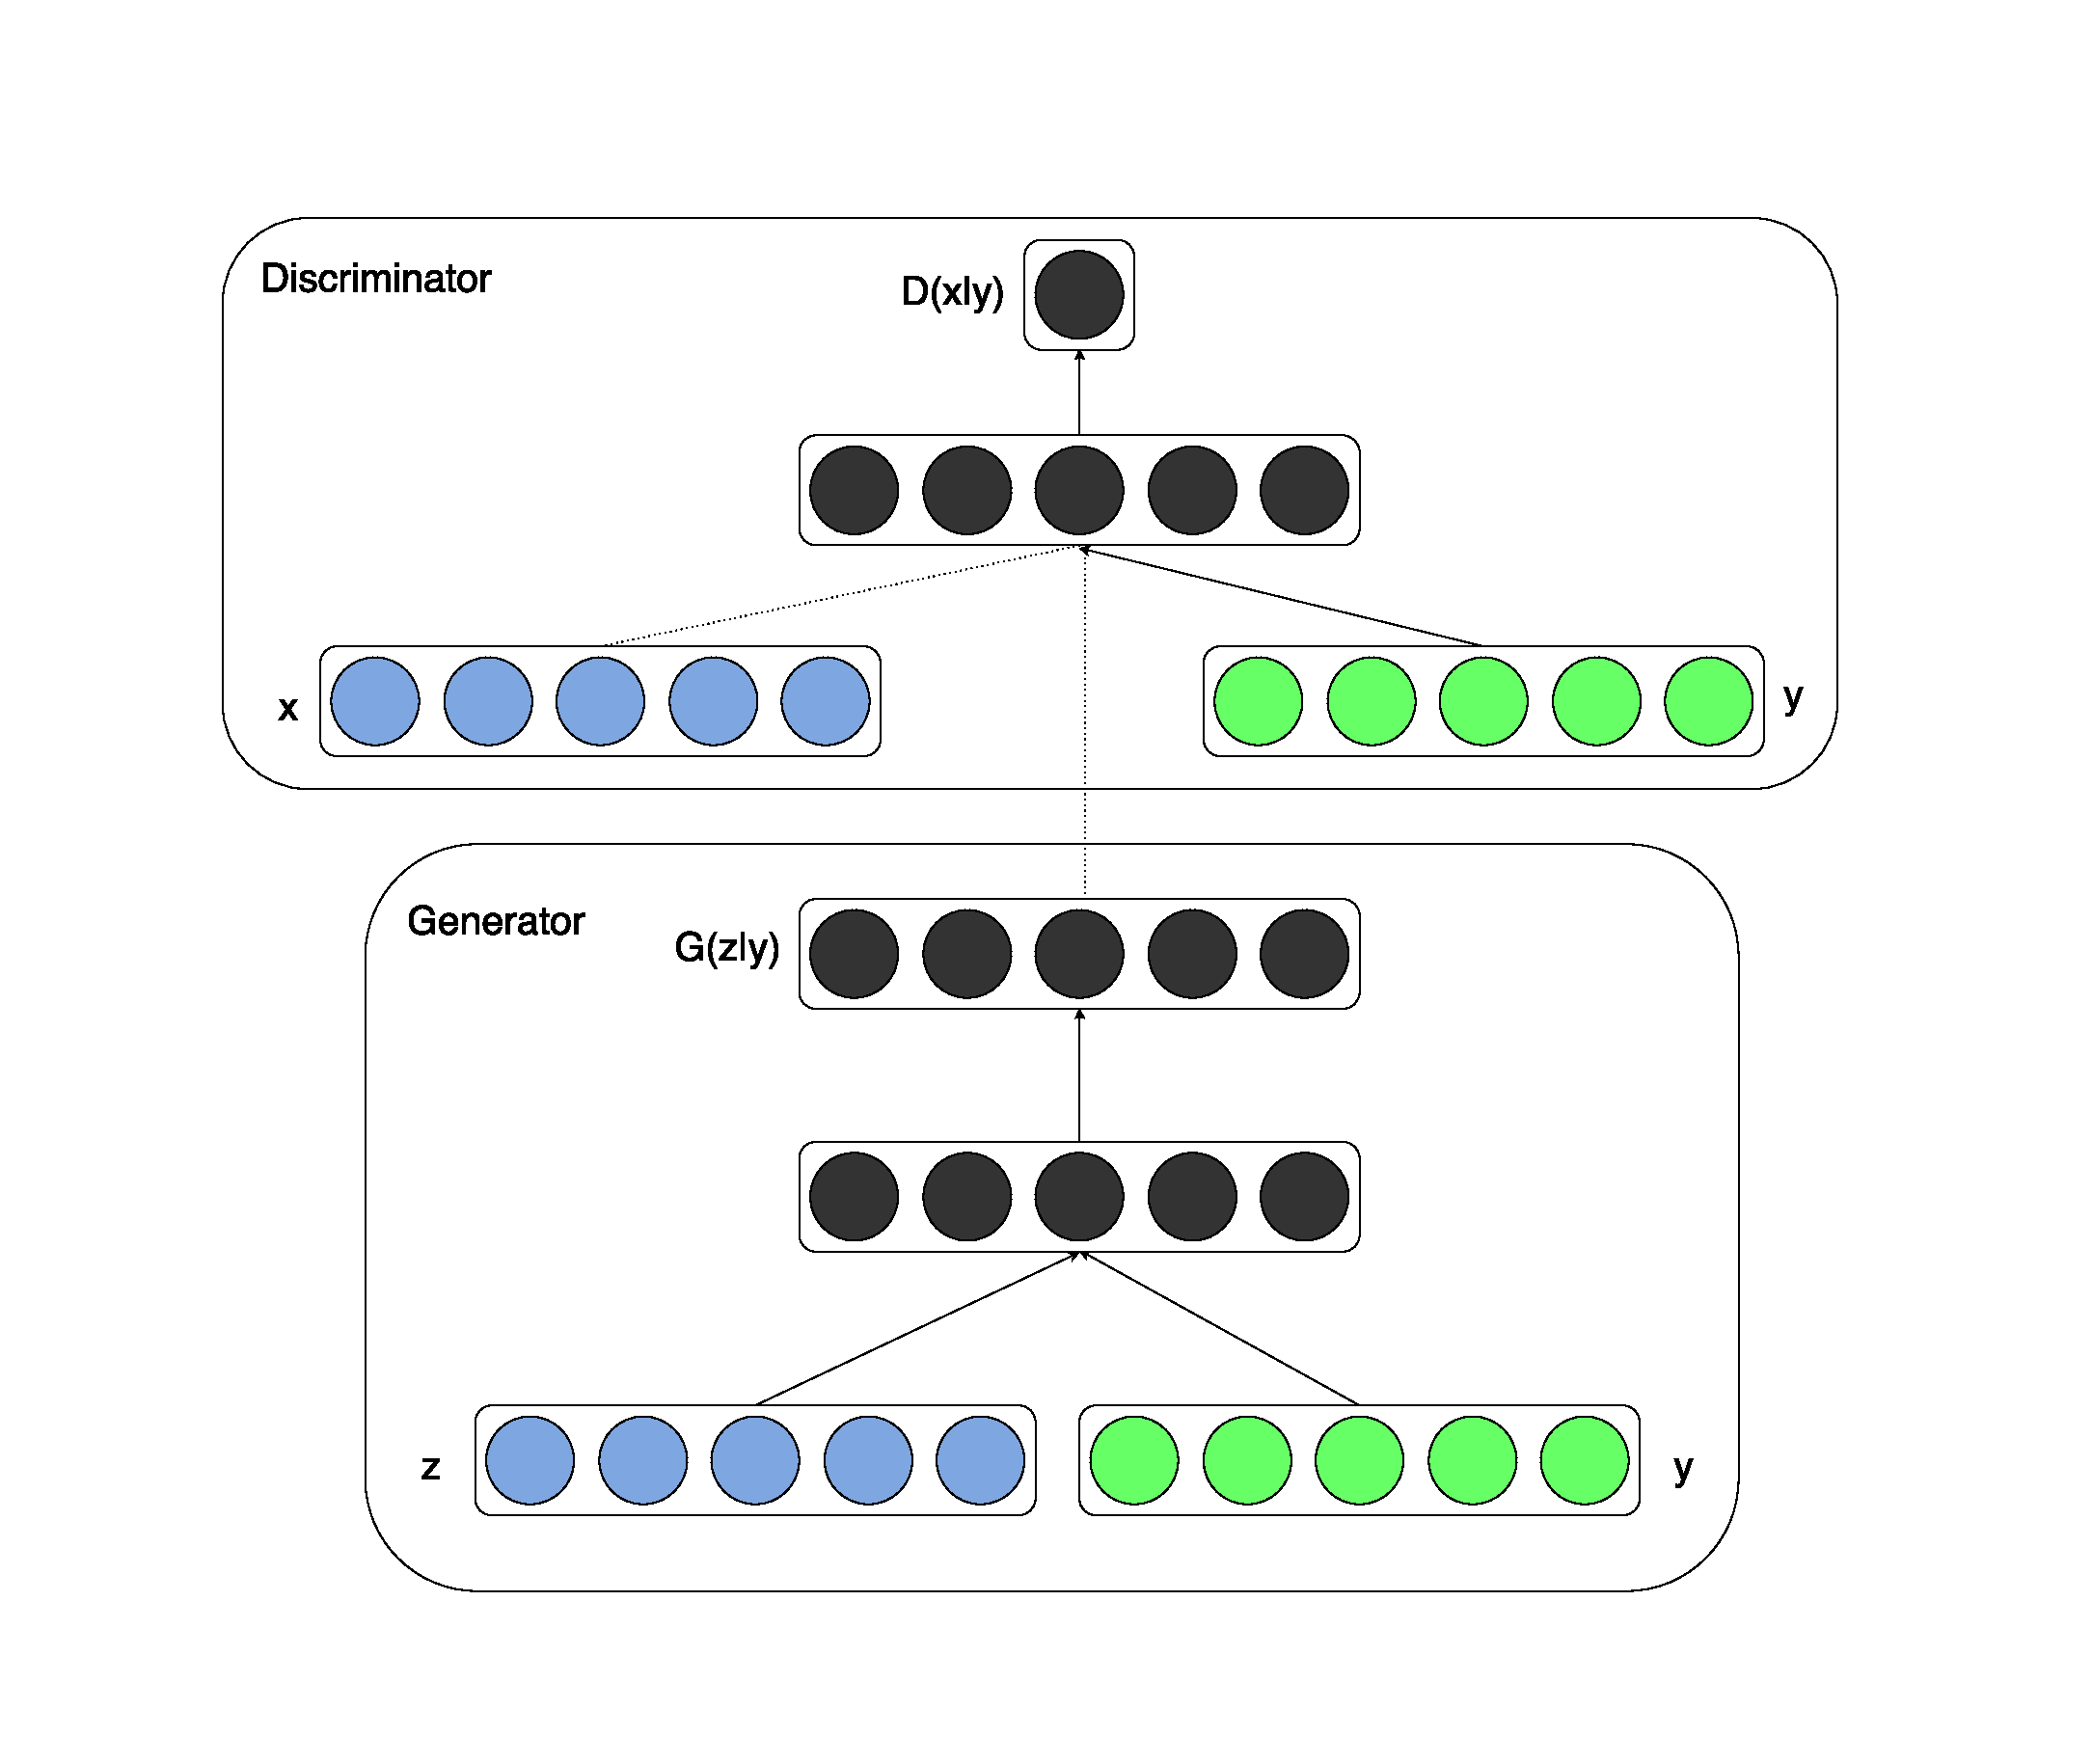
\includegraphics[height=0.85\textheight]{images/diagram.pdf}
		\vspace{-1cm}
		\caption{From \cite{mirzaConditionalGenerativeAdversarial2014}}
	\end{figure}
\end{frame}

\begin{frame}
	\frametitle{Conditional GANs}
	The GANs game becomes:
	$$ 
	\min_G \max_D \underset{x \sim p_{data}(x| \textcolor{red}{y})}{\mathbb{E}} [\log D(x, \textcolor{red}{y})]  +\underset{z \sim p_z(z)}{\mathbb{E}}[\log(1 - D(G(z|\textcolor{red}{y}),\textcolor{red}{y}))]
	$$

	\setbeamercolor{block body}{bg=red!30!white}
	\begin{block}{}
		Notice: the same representation of the condition has to be presented to both network.
	\end{block}
\end{frame}

\begin{frame}[standout]
	GANs Applications
\end{frame}

\begin{frame}[t]
\frametitle{GANs Applications}
	GANs can be applied to different tasks:
	\begin{itemize}
		\only<1>{\item Face generation}
		\only<2>{\item Domain Translation}
		\only<3>{\item Super resolution applications}
	 \end{itemize}
	
	\only<1>{
		\vspace{-0.5cm}
		\begin{figure}
			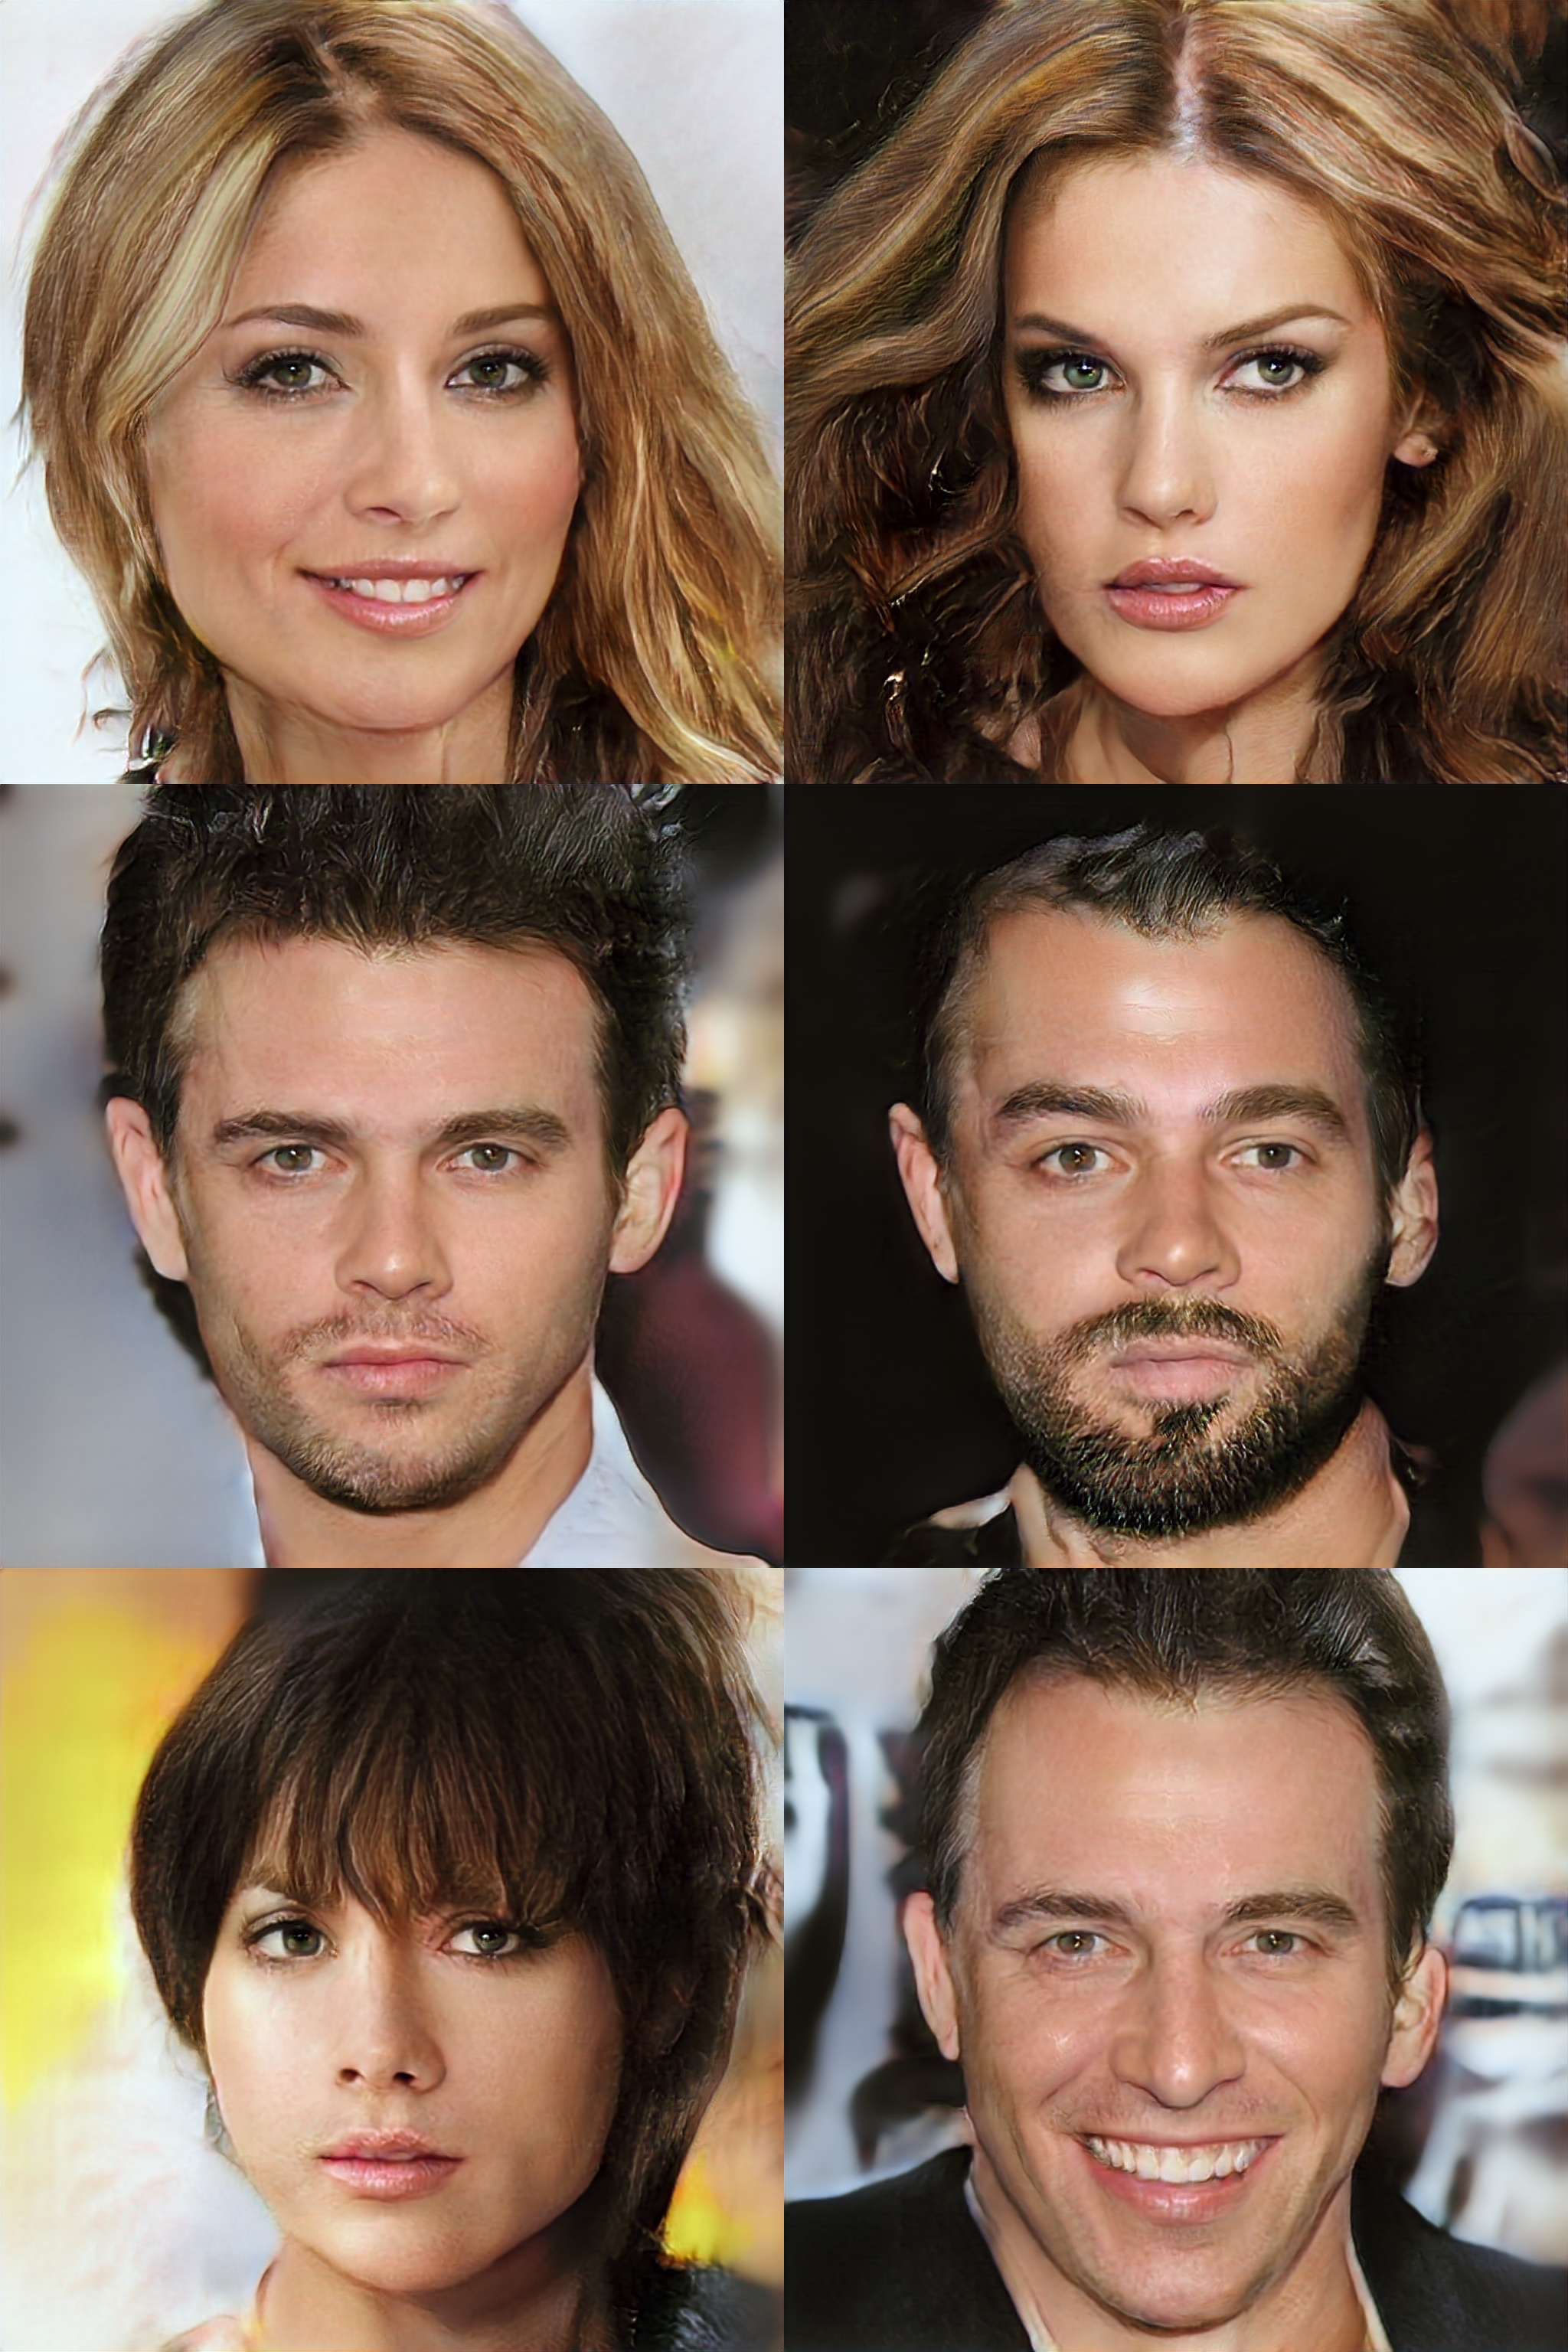
\includegraphics[height=0.7\textheight]{images/incremental.jpg}
			\caption{From \cite{karrasProgressiveGrowingGANs2017}}
		\end{figure}
	}
	\only<2>{
		\begin{figure}
			\centering
			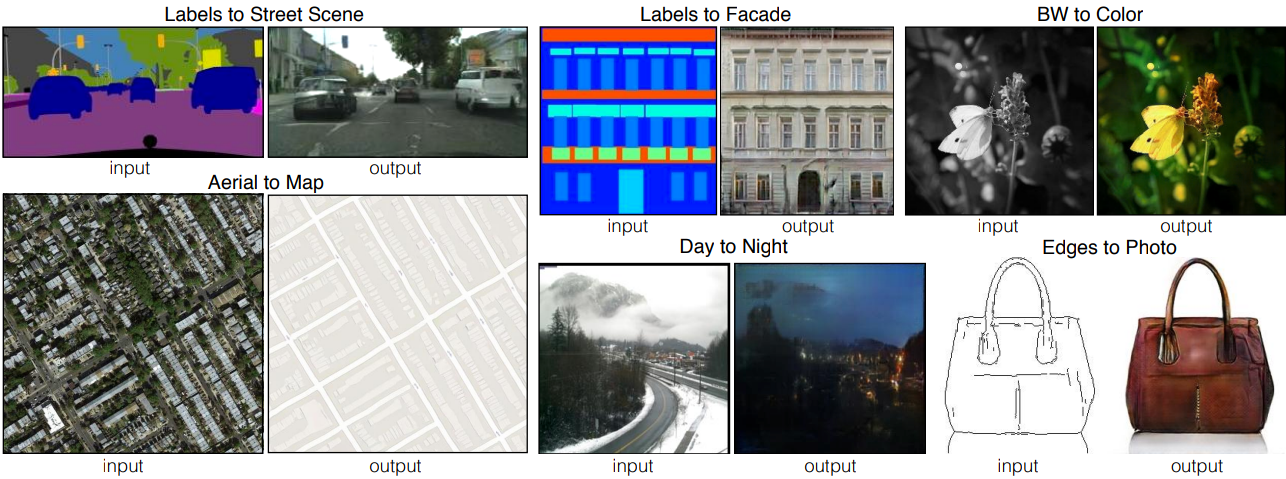
\includegraphics[width=1\textwidth]{images/pix2pix.png}
			\caption{From \cite{isolaImagetoImageTranslationConditional2016a}}
		\end{figure}
	}
	\only<3>{
		\begin{figure}
			\centering
			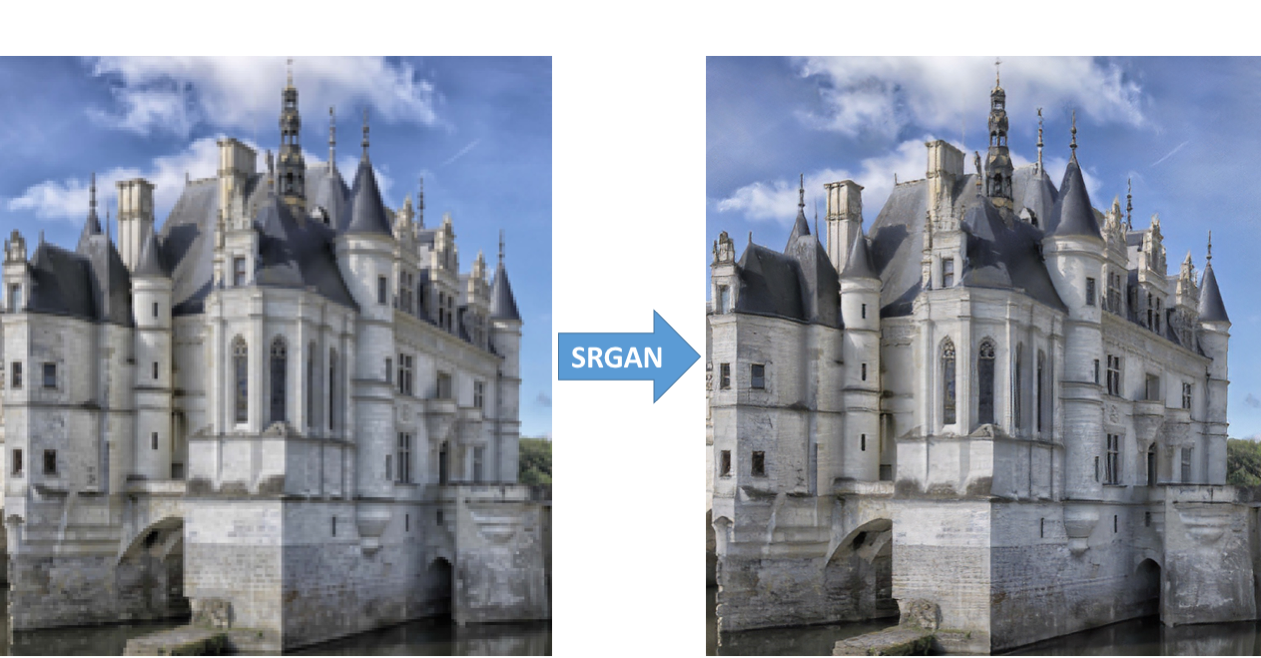
\includegraphics[width=0.9\textwidth]{images/SRGAN.png}
			\caption{From \cite{ledigPhotoRealisticSingleImage2016}}
		\end{figure}
	}
\end{frame}

\begin{frame}[standout]
	\begin{center}
	\Large	Thank you for your attention! \hfill \\
	\Large	Questions?
	\end{center}
\end{frame}

%% reference
\begin{frame}[allowframebreaks]
	 \bibliographystyle{mydinat}
	\bibliography{bibl.bib}
\end{frame}

\end{document}